
\documentclass[pdftex,12pt,xcolor=pdftex,table]{beamer}
\synctex=1
\usepackage{comment}
\usepackage{etex}
\usepackage{amsmath}
\usepackage{amsthm}
\usepackage{amsfonts}
\usepackage{amssymb}
\usepackage{latexsym}
\usepackage{mathtools}
\usepackage[english]{babel}
\usepackage[utf8]{inputenc}
\usepackage{tikz}
\usetikzlibrary{calc,matrix,shapes,arrows}
\usepgflibrary{shapes.arrows}
\usepackage[nomessages]{fp}% http://ctan.org/pkg/fp
\newcounter{mycols}
\usepackage[]{graphicx}
\usepackage[sort]{natbib}
\usepackage{bibentry}
\usepackage{booktabs}
\usepackage{layout}
\usepackage[justification=centering,figureposition=bottom]{caption}
\usepackage{longtable}
\usepackage{lscape}
\usepackage{rotating}
\usepackage[figtopcap,center,scriptsize]{subfigure}%[figtopcap]
\usepackage{appendix}
\usepackage{setspace}
\usepackage[multiple,stable]{footmisc}
\captionsetup[longtable]{width=.75\textwidth}
\usepackage{parskip}
\setlength{\parskip}{\smallskipamount} 
\usepackage{ragged2e}
\usepackage{hyperref}
\DeclareGraphicsExtensions{.png,.pdf}
\DeclareTextFontCommand{\emph}{\bfseries}

%% THEOREMS -------------------------------------------------------
\newtheorem{thm}{Theorem}[section]
\newtheorem{cor}[thm]{Corollary}
\newtheorem{lem}[thm]{Lemma}
\newtheorem{prop}[thm]{Proposition}
\theoremstyle{definition}
\newtheorem{defn}[thm]{Definition}
\theoremstyle{remark}
\newtheorem{rem}[thm]{Remark}
\numberwithin{equation}{section}
%
%% MATH -----------------------------------------------------------
\newcommand{\set}[1]{\left\{#1\right\}}
\newcommand{\eps}{\varepsilon}
\newcommand{\To}{\longrightarrow}

\newcounter{panel}[table]
\renewcommand{\thepanel}{\Alph{panel}}
\newcommand{\mypanel}[1][]{\refstepcounter{panel}Panel \thepanel: \ #1}

\newenvironment{stepenumerate}{\begin{enumerate}[<+->]}{\end{enumerate}}
\newenvironment{stepitemize}{\begin{itemize}[<+->]}{\end{itemize} }
%\newenvironment{stepitemize}{\begin{itemize}}{\end{itemize} }
\newenvironment{stepenumeratewithalert}{\begin{enumerate}[<+-| alert@+>]}{\end{enumerate}}
\newenvironment{stepitemizewithalert}{\begin{itemize}[<+-| alert@+>]}{\end{itemize} }
\newtheorem{assumption}{Assumption}
\newtheorem{proposition}{Proposition}
\usetheme{CambridgeUS}
\setbeamertemplate{navigation symbols}{}
\numberwithin{figure}{section}

\makeatletter
\let\@@magyar@captionfix\relax
\makeatother

\tikzset{arrowcases/.style={matrix anchor=west,%
  nodes={anchor=base west,%
         name=arrc-\the\pgfmatrixcurrentrow-\the\pgfmatrixcurrentcolumn},%
  execute at begin cell=\node\bgroup\math\displaystyle,%
  execute at end cell=\endmath\egroup;,%
  ampersand replacement=\&}}

\def\beginarrowcases#1\endarrowcases{
\begin{tikzpicture}[baseline=(O)]
  \matrix [arrowcases] {
  #1
  };
  \coordinate (A) at (arrc-1-1.west);
  \coordinate (B) at (arrc-\the\pgfmatrixcurrentrow-1.west);
  \coordinate (start) at ($(A)!0.5!(B) - (5em,0)$);
  \foreach \nn in {1,...,\pgfmatrixcurrentrow} {
    \draw[double, -triangle 45,<->] ($(start)+(0,1.5em - \nn em)$) -- (arrc-\nn-1.west);
  };
  \coordinate (O) at ($(start)-(0,0.5ex)$);
  \node at (-1em,0) {};
\end{tikzpicture}}

\makeatother
\setbeamertemplate{footline}
{
  \leavevmode%
  \hbox{%
  \begin{beamercolorbox}[wd=.25\paperwidth,ht=2.25ex,dp=1ex,center]{author in head/foot}%
    \usebeamerfont{author in head/foot}\insertshortauthor
  \end{beamercolorbox}%
  \begin{beamercolorbox}[wd=.4\paperwidth,ht=2.25ex,dp=1ex,center]{title in head/foot}%
    \usebeamerfont{title in head/foot}\insertshorttitle
  \end{beamercolorbox}%
  \begin{beamercolorbox}[wd=.35\paperwidth,ht=2.25ex,dp=1ex,center]{date in head/foot}%
  \insertshortdate{}\hspace*{3ex}
    \insertframenumber{} / \inserttotalframenumber\hspace*{1ex}
  \end{beamercolorbox}}%
  \vskip0pt%
}
\makeatletter

\title[Natural Selection on Infectious Disease]{The Natural Selection on Infectious Disease Resistance and It's effect on contemporary Health}
\subtitle{\footnotesize{by C. Justin Cook}}
\institute{Economic Growth and Comparative Development}
\author{Sara Ariza  \\ & Laura V. León}
\centering
\date{June 18 2020}


\makeatletter
\@addtoreset{subfigure}{figure}
\makeatother
\makeatletter \@addtoreset{subfigure}{framenumber} \makeatother

\begin{document}

\begin{frame}%[plain]
\titlepage
\end{frame}

\begin{frame}
\frametitle{Table of Contents}
\tableofcontents
\end{frame}


\begin{frame}\section{About the author}
\justifying
\frametitle{About the author}
\framesubtitle{C. Justin Cook}
\url{https://cjustincook.weebly.com/}\\~\\
\thinspace
Assistant Professor of Economics at University of California, Merced.\\&\\

\includegraphics[height=5cm]{autor.jpg}
\centering
\end{frame}


\begin{frame}
\frametitle{About the author}
\framesubtitle{C. Justin Cook}
\justifying
Interests:
\begin{itemize}
    \item Economic Growth.
    \item Health.
    \item Development.
    \item Macrogenoeconomics.
\end{itemize}\\

Education:
\begin{itemize}
    \item Louisiana State University, Baton Rouge, LA USA.
    \begin{itemize}
        \item Ph.D., Economics, 2012. Dissertation (Advisor: Areendam Chanda): Investigating the Role of Genetic Variation in
Explaining Long Run Economic Outcomes
       \item M.S., Economics, 2009.
       \item B.S., Economics (Concentration in Empirical Studies), 2006.

    \end{itemize}
\end{itemize}
\end{frame}

\begin{frame}{Abstract}
\justifying
 \textit{“This paper empirically tests the association between genetically determined resistance to infectious disease and cross-country health differences. A country-level measure of genetic diversity for the system of genes associated with the recognition and disposal of foreign pathogens is constructed. Genetic diversity within this system has been shown to reduce the virulence and prevalence of infectious diseases and is hypothesized to have been naturally selected from historical exposure to infectious pathogens. Base estimation shows a statistically strong, robust, and positive relationship between this constructed measure and country-level health outcomes in times prior to, but not after, the international epidemiological transition.”}
 
\end{frame}
\section{Introduction}
\begin{frame}
\frametitle{Introduction}
    \justifying
    Prior to the major medical discoveries associated with the international epidemiological transition, infectious diseases were a major determinant of mortality and subsequent differences in life expectancy across countries. 
\justifying
\pause
\begin{itemize}

    \item The discovery and widespread use of effective medicines in the late 1940s to early 1950s is labeled by (Acemoglu\&Johnson, 2007)\cite{acemoglu2007disease} as the international epidemiological transition.
    \pause
    \item In 1940, the average cross-country life expectancy at birth was 47 years with a standard deviation of 12 years; however, for 1980 the average life expectancy grew to 66 years, and the standard deviation across countries fell to 9 years. 

\end{itemize}

\end{frame}

\begin{frame}
\frametitle{Introduction}
\justifying
  \begin{block}{Question?}
What were the causes of the initial cross-country disparities in the virulence of infectious diseases?
\end{block}
\pause
\begin{block}{Hypothesis}
Innate resistance did influence country-level response to infectious disease prior to the international epidemiological transition, however, the effects of innate resistance are dissipated by more efficacious health technologies.

\end{block}
\end{frame}

\begin{frame}{Introduction}
\begin{block}{The HLA system}
\justifying
The measure of genetic resistance is  found within the human leukocyte antigen (HLA) system. The HLA is responsible for locating foreign proteins in order to direct cells of the immune system to initiate an immune response and is broken into two major classes, class I and class II, with both classes being associated with the recognition of certain pathogens (Piertney\&Oliver, 2006)\cite{piertney2006evolutionary}.
\pause
\end{block}

\begin{itemize}
    \item
Using country-level aggregations of ethnic-level genetic data, the author constructs a cross-country measure for diversity within the HLA system: HLA heterozygosity .
\end{itemize}
\pause
\begin{itemize}
    \item \textbf{HLA heterozygosity or  Expected heterozygosity} is defined as the probability that two randomly selected individuals differ in regard to genetic variants, or alleles, for a particular locus. 

\end{itemize}

\end{frame}
\section{Background}
\begin{frame}
\frametitle{Background}
\framesubtitle{Historic Differences in Infectious Disease Environments}
\justifying
The number of infectious diseases humans face increased substantially with the introduction of agriculture, commonly referred to as the \textbf{Neolithic revolution} (Wolfe, Dunavan\&Diamond 2007)\cite{wolfe2007origins}
\pause
\begin{itemize}
    \item Agriculture allowed the development of large, dense, and sedentary populations.
    \pause
    \item The domestication of animals in the Neolithic provided closer contact between animals and humans.
    \pause
\end{itemize}
The timing of the Neolithic revolution is associated with contemporary differences across populations in genetic diversity within the HLA system.
\end{frame}


\begin{frame}{Background}
\framesubtitle{The Natural Selection of HLA Heterozygosity}
\justifying
The set of genes comprising the HLA system represents one of the most genetically diverse regions of the \textbf{genome} (Jeffery \& Bangham, 2000) \cite{jeffery2000infectious}.
\pause
\begin{itemize}
    \item This high level of diversity is hypothesized to have been naturally selected as a mechanism of resistance to infectious pathogens (Hughes\&Yeager, 1997)\cite{hughes1998natural} (Penman et al., 2013)\cite{penman2013pathogen} (Spurgin\&Richardson, 2010)\cite{spurgin2010pathogens}.
    \pause
   \item This natural selection for diversity within the HLA system is from balancing selection.
   \pause
    \item Balancing selection results from two distinct reasons (Slade\&McCallum, 1992)\cite{slade1992overdominant}:
    \begin{itemize}
        \item Overdominance.
        \item Frequency dependence.

    \end{itemize}
\end{itemize}
\end{frame}

\begin{frame}{Background}
\framesubtitle{Out-of-Africa Migration and Genetic Diversity}
\justifying
The overall level of genetic diversity within a population has recently been shown to be a function of the population’s migratory distance from East Africa (Ashraf & Galor, 2013)\cite{ashraf2013out} (Ramachandran et al., 2005)\cite{ramachandran2005support}. 
\pause
\begin{itemize}
    \item Modern human populations originated within East Africa (roughly Ethiopia) and subsequently migrated to all other continents, excluding Antarctica.
    \pause
    \item Given that the entire set of genetic diversity was contained within the initial East African population and that migrating populations contain only a subset of this diversity, a strong, negative, and linear association exists between the distance along migration routes a country is from East Africa and the genomic diversity of populations within a country.
\end{itemize}
\end{frame}


\section{Data}
\begin{frame}
\frametitle{Data}
\framesubtitle{HLA Heterozygosity}
\justifying
Ashraf and Galor (2013; hereafter AG)\cite{ashraf2013out} explore the role of genetic variation in explaining historical and contemporary levels of development. In order to measure genetic diversity, they use the expected heterozygosity, roughly defined as: “the probability that two randomly selected individuals differ with respect to the gene in question” (AG, p. 3).
\pause
\begin{itemize}
    \item Expected heterozygosity is calculated with the frequency of gene variants, or alleles, at a particular site on the genome, or locus:
    \pause
\end{itemize}
\begin{equation}
    H_{exp}=1-\frac{1}{m}\sum^{m}_{l=1}\sum^{kl}_{l=1}p_{i}^{2}
\end{equation}
\pause
Where:\\
$pi$ represents the fraction of allele $i$ within each population and expected heterozygosity is found by the average across $m$ loci.
\end{frame}


\begin{frame}{Data}
\framesubtitle{The author measures of interest is referred to as HLA heterozygosity.}
\justifying

\begin{itemize}
\item This measure intends to capture balancing selection within the HLA system from historical exposure to infectious pathogens and is not representative of the entire genoma.
\pause
\item HLA heterozygosity is constructed with data on SNPs from the Allele Frequency Database at Yale University, referred to as ALFRED (Kidd et al., 2003)\cite{kidd2003alfred}.
\pause
\item A SNP (single-nucleotide polymorphism) is a single change along a strand of DNA. 
\pause
\item ALFRED provides allele frequencies for anthropologically defined ethnicities, providing genetic data for 156 SNPs within 19 HLA genes for 51 distinct ethnic groups. These ethnic data are then aggregated to the country level by matching ethnic compositions within (Alesina et al., 2003)\cite{alesina2003fractionalization} 

\end{itemize}
\end{frame}


\begin{frame}{Data}
\framesubtitle{HLA Heterozygosity}
\justifying

\begin{itemize}
\item The country-level measure of HLA heterozygosity is the weighted average of ethnic-level HLA heterozygosities, where weights are determined by the fraction of the contemporary population associated with each ethnicity.
\pause
\item Through this method, the author constructed genetic diversity scores for 175 countries, of which 131 are used in the baseline regression model. 
\end{itemize}
\end{frame}

\begin{frame}{Data}
\framesubtitle{HLA Heterozygosity}
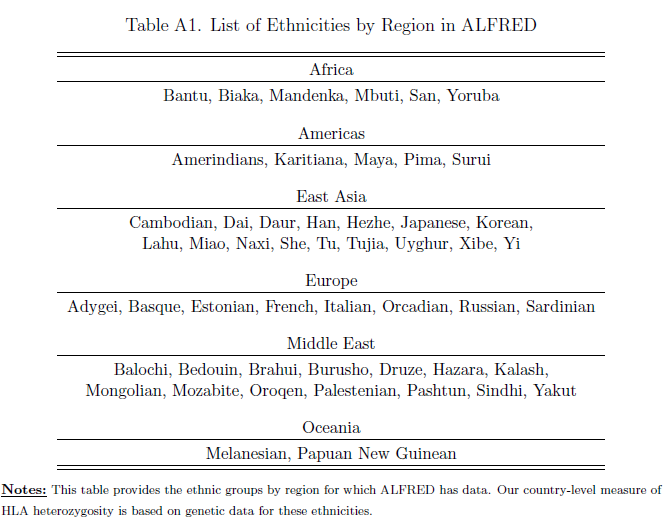
\includegraphics[height=7cm]{Appendix_1.PNG}
\centering
\end{frame}

\begin{frame}{Data}
\framesubtitle{Health Outcomes prior to the International Epidemiological Transition}
\justifying
\begin{itemize}
\item The author consider a number of country-level health outcomes prior to the discovery and diffusion of medical technologies associated with the international epidemiological transition.
\pause
\item These include both predicted mortality from infectious disease and life expectancy in 1940, as well as life expectancy in 1960.
\pause
\item The use of 1940s data, while truly before the epidemiological transition, is problematic due to a lack of data in relatively poor countries, leading to possible selection bias. Therefore, the primary dependent variable is country level life expectancy at birth in 1960

\end{itemize}
\end{frame}

\begin{frame}{Data}
\framesubtitle{HLA Heterozygosity}
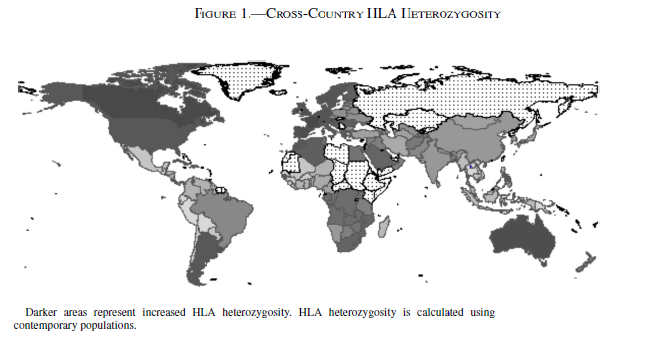
\includegraphics[height=7cm]{Figure_1.png}
\centering
\end{frame}


\section{Results}
\begin{frame}
\frametitle{Results}
\framesubtitle{Explaining HLA Heterozygosity}
\justifying
\textit{Table 1} shows the summary statistics for : \textit{i)} HLA heterozygosity and \textit{ii)} the overall level of genetic diversity from (Ashraf\&Galor, 2013)\cite{ashraf2013out}.\\ 
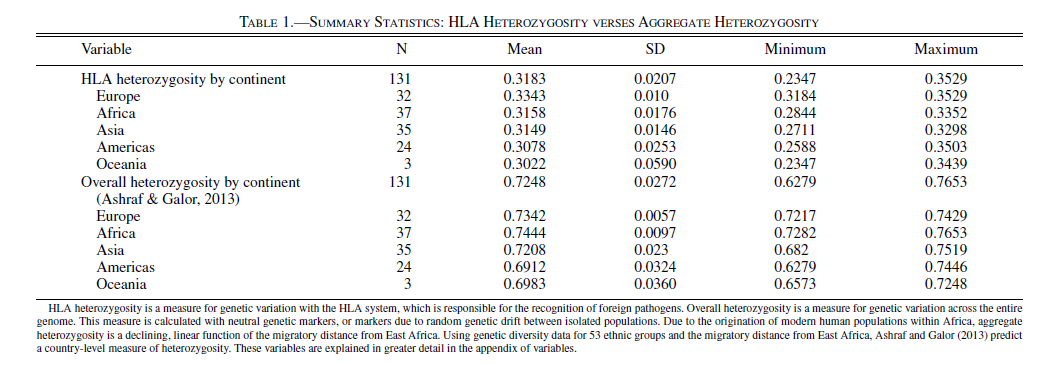
\includegraphics[height=4cm]{Table_1.PNG}

\justifying
Acording to the results, African countries are found to have the highest levels of overall diversity, while countries from Europe contain the greatest amount of diversity within the HLA system.
\end{frame}

\begin{frame}{Results}
\framesubtitle{Explaining HLA Heterozygosity}
\justifying
\textit{Figure 2} plots the measure of diversity, HLA heterozygosity, as a linear function of migratory distance from East Africa. 
\\ 
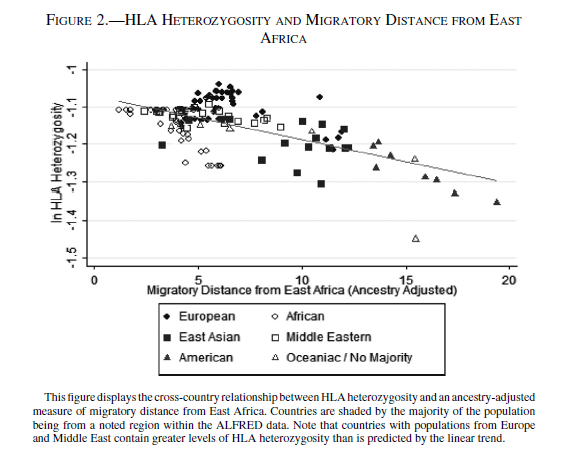
\includegraphics[height=6cm]{Figure_2.PNG}
\centering
\end{frame}

\begin{frame}{Results}
\framesubtitle{Explaining HLA Heterozygosity}
\justifying
From \textit{figure 2}, countries with a majority population from Europe and the Middle East tend to break from the linear association between HLA heterozygosity and migratory distance from East Africa, containing higher-than-predicted levels of HLA heterozygosity.\\~\\
The role of both the migratory distance from East Africa and the Neolithic revolution in explaining HLA heterozygosity is tested in \textit{table 2}.
\end{frame}

\begin{frame}{Results}
\framesubtitle{Explaining HLA Heterozygosity}
\justifying
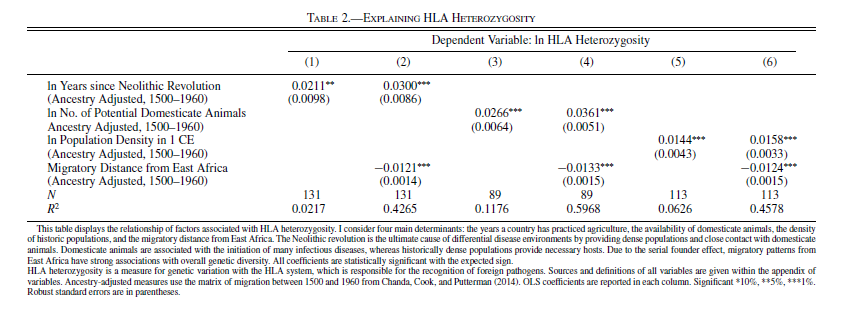
\includegraphics[height=4.5cm]{Table_2.PNG}
\end{frame}


\begin{frame}{Results}
\framesubtitle{HLA Heterozygosity, Country-Level Health Outcomes, and the International Epidemiological Transition}
\justifying
Equation used to test that genetic resistance to infectious disease, measured by HLA heterozygosity, is positively associated with country-level health outcomes prior to the international epidemiological transition.,
\pause
\begin{equation}
    \ln y_{i}^{t<i.e.t.}=\alpha+\beta_{1}(\ln HLA_{i})+\boldsymbol{\beta}_{2}'\mathbf{X_{i}}+\boldsymbol{\beta}_{3}'\mathbf{I_{i}^{c}}+\epsilon_{i}
\end{equation}

\end{frame}

\begin{frame}{Results}
\framesubtitle{HLA Heterozygosity, Country-Level Health Outcomes, and the International Epidemiological Transition}
\justifying

\centering
    $\ln y_{i}^{t<i.e.t.}=\alpha+\beta_{1}(\ln HLA_{i})+\boldsymbol{\beta}_{2}'\mathbf{X_{i}}+\boldsymbol{\beta}_{3}'\mathbf{I_{i}^{c}}+\epsilon_{i}$
\pause
\begin{itemize}
\item \mathbf{$i$}: is a country indicator.
\item \bold{$yt\leq i.e.t.$}: i represents aggregate health outcomes prior to the international epidemiological transition.
\item \textbf{$\beta_{1}$}: measures the effect of HLA heterozygosity.
\item $X_{i}$: is a vector of country-level controls, including ethnic fractionalization, agricultural productivity, geography, and an ancestry-adjusted measure for the agricultural transition.
\item $I^{c}_{i}$: is an indicator variable as to whether country i is within continent c.
 \item {$\epsilon_{i}$}: is the cross-country error term. 
\end{itemize}
\end{frame}


\begin{frame}{Results}
\framesubtitle{Explaining HLA Heterozygosity}
\justifying
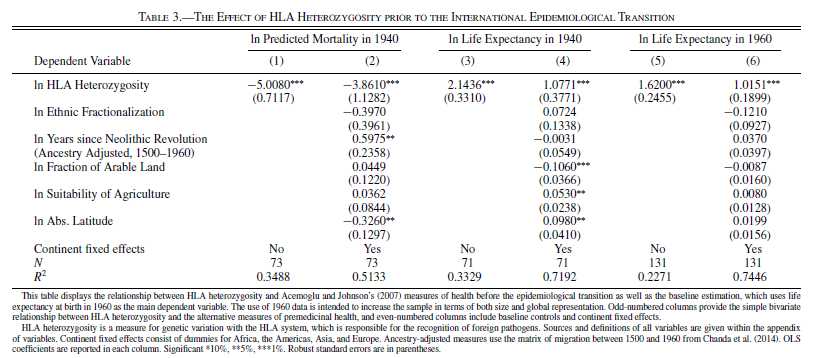
\includegraphics[height=5.45cm]{Table_3.PNG}
\end{frame}

\begin{frame}{Results}
\framesubtitle{HLA Heterozygosity, Country-Level Health Outcomes, and the International Epidemiological Transition}
\justifying
The Estimates in \textit{table 3} consider three alternatives for measuring country-level health outcomes prior to the epidemiological transition: 
\pause
\begin{itemize}
    \item The mortality rate from fifteen infectious diseases in 1940.
    \pause
    \item Life expectancy at birth in 1940.
    \pause
    \item Life expectancy at birth in 1960.
\end{itemize}
\end{frame}


\begin{frame}{Results}
\framesubtitle{HLA Heterozygosity, Country-Level Health Outcomes, and the International Epidemiological Transition}
\justifying
\textit{Table 4} explores the effect of HLA heterozygosity on life expectancy from 1960 to 2010 and tests the effect of HLA heterozygosity, or innate resistance, in post epidemiological transition environments. It shows that 1960 is an early enough period to capture the effects of innate resistance.\\
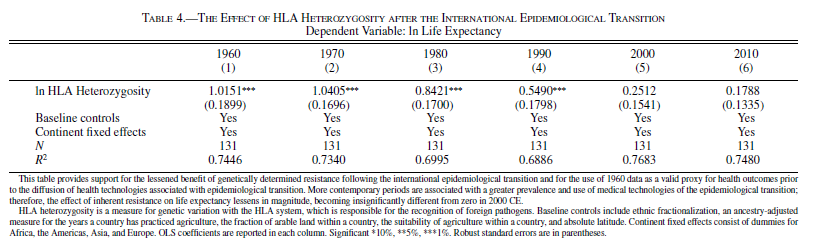
\includegraphics[height=3.5cm]{Table_4.PNG}
\end{frame}


\begin{frame}{Results}
\framesubtitle{HLA Heterozygosity, Country-Level Health Outcomes, and the International Epidemiological Transition}
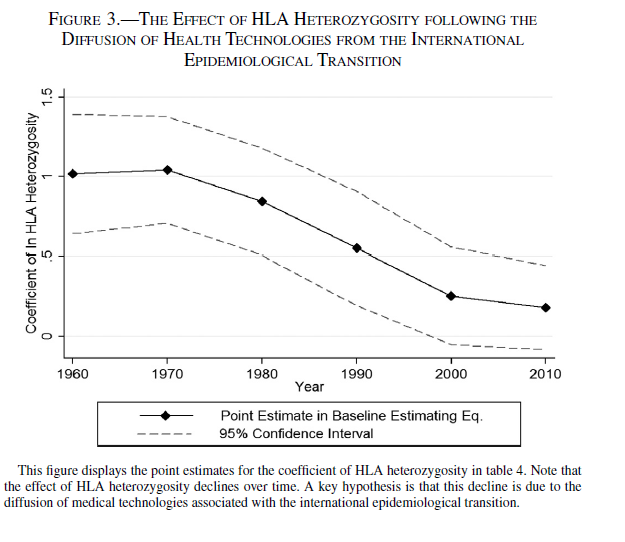
\includegraphics[height=6cm]{Figure_3.PNG}
\end{frame}


\begin{frame}{Results}
\framesubtitle{Robustness}
\justifying
\textbf{Controlling for regional ethnic differences.}\\
The relationship between HLA heterozygosity and life expectancy in 1960 may reflect some underlying role of European populations in promoting greater health outcomes. In addition, other populations may have unobserved effects that are also correlated with both HLA heterozygosity and life expectancy in 1960.\\ 
\pause
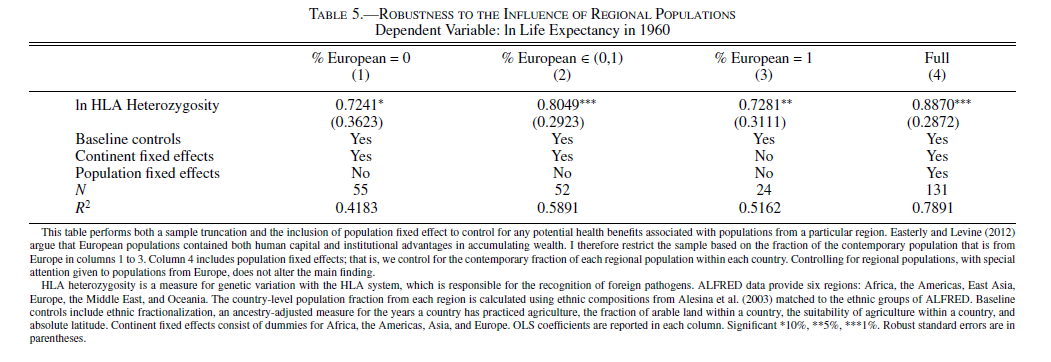
\includegraphics[height=4cm]{Table_5.PNG}
\end{frame}

\begin{frame}{Results}
\framesubtitle{Robustness}
\justifying
\textbf{Omitted variables.}\\
The author includes omitted variables that may be associated with either the measure of HLA heterozygosity or life expectancy in 1960.\\
\pause
The additional variables are broken into two classes:
\pause
\begin{itemize}
    \item Exogenous: Include genetic, geographic, and historic population controls \textit{(Table 6)}.
    \pause
    \item  Endogenous: Consist of income, human capital, and demographics in 1960 \textit{(Table 7)}.
\end{itemize}
\end{frame}

\begin{frame}{Results}
\framesubtitle{Robustness}
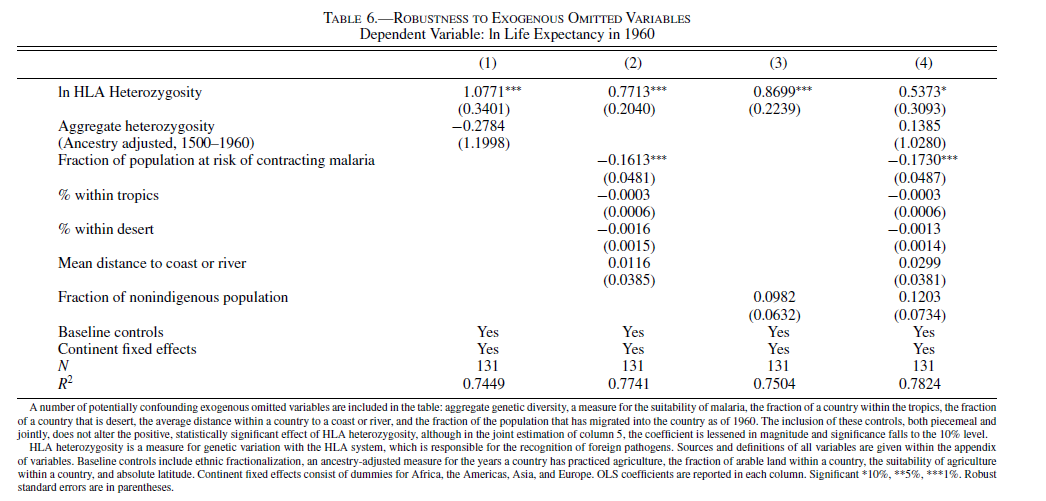
\includegraphics[height=6cm]{Table_6.PNG}
\end{frame}

\begin{frame}{Results}
\framesubtitle{Robustness}
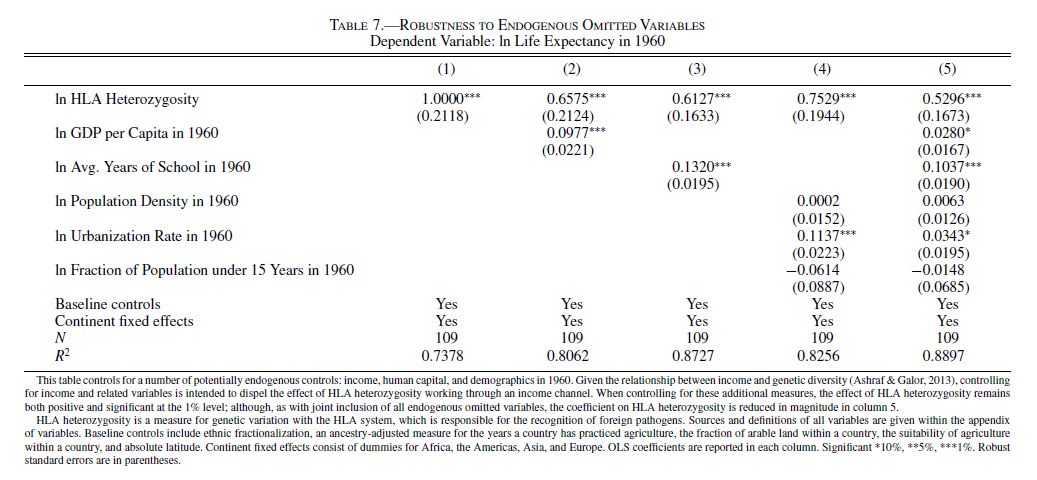
\includegraphics[height=5.5cm]{Table_7.PNG}
\end{frame}

\section{Conclusion}
\begin{frame}
\frametitle{Conclusion}
\begin{itemize}
    \item HLA heterozygosity has a positive, statistically significant, and robust relationship with life expectancy at birth in 1960, a period argued to be before the diffusion of health technologies associated with the international epidemiological transition.
    \pause
    \item The strong statistical relationship between HLA heterozygosity and life expectancy is substantially lessened by the introduction of medicines and vaccines, which dissipate any benefits from genetically determined resistance.
    \pause
    \item An important source of the variation in HLA heterozygosity is the differential timing date of the Neolithic revolution, which provided the means of development for a much more severe infectious disease environment.
    
\end{itemize}
\end{frame}

\section{Bibliography}
\begin{frame}
\frametitle{Bibliography}
\begin{itemize}
    \item 
Cook, C.J. (2015). The natural selection of infectious disease resistance and its effect on contemporary health.  The Review of Economics and Statistics, 97, 742-757.

\end{itemize}
\end{frame}

\begin{frame}{References}
\tiny{
     \bibliographystyle{ieeetr}
  \bibliography{bibliografia1}
}
    
\end{frame}

\begin{frame}{Contact information}
    \begin{block}{Sara Ariza Murillo}
    Economist, Universidad del Rosario.\\
    email: \url{saraariza97@gmail.com}
    \end{block}
   \begin{block}{Laura Viviana León Díaz}
    Finance and International Trade, Universidad del Rosario.\\
    email: \url{leond.laura@gmail.com}
    \end{block}      
    
\end{frame}


\end{document}


